\setdictum{%
  Money. A social life. A shave.\\
  A Ph.D.\ student needs not such things.%
}{%
  Mike Slackenerny
  (PHD Comics\footnotemark)%
}

\longchapter{%
  Application 1: Topology Optimization%
}{%
  Application 1:\texorpdfstring{\\}{ }Topology Optimization%
}{%
  Application 1 -- Topology Optimization%
}
\footnotetext{\url{http://phdcomics.com/comics/archive.php?comicid=40}}
\label{chap:60topoOpt}

\initial{0em}{N}{ow, we want to investigate}
the first real-world application,
which is the field of topology optimization.
The classical and widely-used method in engineering is shape optimization,
where the shape of a component
(parameterized by $\*x \in \real^d$) has to be
determined such that some objective function value $\objfun(\*x)$ is optimal,
i.e., minimal or maximal.
For example, a bridge over a valley can be built in the shape of a
parabolic arc.
The task of shape optimization is then to choose the coefficients of the
parabola such that the bridge's stability is maximized,
possibly with the constraint that the volume occupied by the bridge
does not exceed a certain value (to save construction costs) or
that the size of the resulting passage meets some size requirements
(e.g., at least \SI{20}{\meter} wide and \SI{6}{\meter} tall).

However, the framework of shape optimization unnecessarily prescribes the
topology of the shapes in the search space \cite{Allaire16Towards}.
In the bridge example, it may well be that a viaduct-type bridge with
three arcs instead of one is more stable while occupying less volume.
We are not able to find such a bridge with shape optimization
in the previous example,
as we have restricted the search space to single-arc bridges.
This issue is resolved by the more sophisticated
framework of topology optimization, where the topology%
\footnote{%
  Two objects are considered ``topologically different''
  if their numbers of ``holes'' differ.
  This stems from the fact that in the field of mathematical topology,
  the \term{genus} (i.e., the number of holes)
  of a topological space is a \term{topological invariant,} i.e.,
  the genus is invariant under homeomorphism.
  If the genera of two topological spaces differ, then they cannot be
  homeomorphic and are thus considered topologically different.%
}
is not given by the user,
but chosen by the optimization algorithm (in a hopefully optimal way),
rendering topology optimization a key area of simulation technology.

Recently, B-splines have been used for
shape optimization \cite{Martin16Formoptimierung} and
topology optimization \multicite{Qian13Topology,Zhang17Topology}.
Sparse grids have been employed for
topology optimization \cite{Huebner14Mehrdimensionale} as well.
In this chapter, we want to combine these two numerical tools,
which have been used in isolation until now,
to perform topology optimization using B-splines on sparse grids.
The two most common approaches for topology optimization are
the \term{level-set method} and
the \term{homogenization method} \cite{Allaire16Towards}.
The level-set method describes the boundary of the object
as the zero level set $\psi^{-1}(0)$ of a function
$\psi\colon \objdomain \to \real$ \term{(level-set function)}
and uses a \pde to iteratively transport this function and,
consequently, the object's boundary \cite{Allaire04Topology}.
However, we want to focus on the second method:
the method of homogenization.

This chapter is structured as follows:
\Cref{sec:61homogenization} explains the homogenization method.
In \cref{sec:62tensors}, we discuss the details of applying B-splines on
sparse grids to this method.
We set up different micro-cell models and scenarios in \cref{sec:63models},
before reviewing numerical results in \cref{sec:64results}.
The results in this chapter have been obtained in collaboration with
Prof.\ Dr.\ Michael Stingl and Daniel Hübner
(both FAU Erlangen-Nürnberg, Germany).
The author of this thesis contributed the parts related to
interpolation and sparse grids, while the collaborators at FAU
studied the engineering and application parts of the joint project
(for example, they provided optimization scenarios and
assessed the quality of the results).

\section{Homogenization and the Two-Scale Approach}
\label{sec:61homogenization}

\minitoc{70mm}{4}

\noindent
We roughly follow the presentation given in
\multicite{%
  Huebner14Mehrdimensionale,%
  Valentin14Hierarchische,%
  Valentin16Hierarchical%
}.
The necessary notation is summarized in
\cref{tbl:glossaryTopologyOptimization}.

\begin{table}
  \setnumberoftableheaderrows{0}%
  \newcommand*{\pnst}[1]{\printnotationsymbol{#1}&\printnotationtext{#1}}%
  \begin{tabular}{%
    >{\kern\tabcolsep}=l<{\kern-1.5mm}+l<{\kern2.9mm}+l<{\kern-1.5mm}+l%
    <{\kern2.9mm}+l<{\kern-1.25mm}+l<{\kern\tabcolsep}%
  }
    \toprulec
    \pnst{\objdomain}&       \pnst{\force}&        \pnst{\densglobal}\\
    \pnst{\dimobjdomain}&    \pnst{\displacement}& \pnst{\denscell}\\
    $d$&\#micro-cell param.& \pnst{\compliance}&   \pnst{\densub}\\
    \pnst{\mcp}&             \pnst{\vol}&          \pnst{\etensor}\\
    &&                       \pnst{\voldens}&      \pnst{\cholfactor}\\
    \bottomrulec
  \end{tabular}%
  \caption[Glossary for topology optimization]{%
    Glossary of the notation for topology optimization.%
  }%
  \label{tbl:glossaryTopologyOptimization}%
\end{table}



\subsection{Homogenization}
\label{sec:611homogenization}

\paragraph{Density function}

Let $\objdomain \subset \real^{\dimobjdomain}$ be the object domain.%
\footnote{%
  We use tildes to denote variables and quantities
  that correspond to the object domain $\objdomain$
  (e.g., $\tilde{\*x}$ is a point in $\objdomain$).
  In contrast, variables without a tilde will correspond
  to the sparse grid domain $\clint{\*0, \*1} = \clint{0, 1}^d$
  (e.g., $\gp{\*l,\*i} \in \clint{\*0, \*1}$ will be a sparse grid point).%
}
Usually, we assume $\dimobjdomain = 2$ or $\dimobjdomain = 3$,
although the method can be generalized to
arbitrary dimensionalities $\dimobjdomain \in \nat$.
Shapes and topologies are described by \term{density functions}
$\densglobal\colon \objdomain \to \clint{0, 1}$.
The function values $\densglobal(\tilde{\*x}) \in \clint{0, 1}$
tell if $\tilde{\*x}$ is contained in the object (value of one) or
not (value of zero).
The \term{homogenization} approach also allows values between
zero and one, giving the physical density of the material in $\tilde{\*x}$.

\paragraph{Optimization of compliance values}

Furthermore, for every density function $\densglobal$,
let $\compliance(\densglobal)$ be an objective function value.
In our setting, which is shown in \cref{fig:topoOptExample},
we exert a force $\force$ on the object,
measure the resulting deformation, and
compute the \term{compliance} (i.e., the inverse of the stiffness) as
the objective function value~$\compliance(\densglobal)$:
\begin{equation}
  \compliance(\densglobal)
  = \int_{\objdomain} \tr{\force} \displacement_{\densglobal}(\tilde{\*x})
  \diff\tilde{\*x},
\end{equation}
where the \term{displacement function}
$\displacement_{\densglobal}\colon \objdomain \to \real^{\dimobjdomain}$
depends on the density \cite{Huebner14Mehrdimensionale}.
We want to find the density function
with the minimal compliance value:
\begin{equation}
  \label{eq:topoOptProblemContinuous}
  \min_{\densglobal}\, \compliance(\densglobal).
\end{equation}
If we do not impose additional conditions,
then there are often uninteresting trivial solutions.
For example, choosing $\densglobal :\equiv 1$
(i.e., filling the entire domain $\objdomain$ with material)
usually leads to the topology with the
highest stiffness and, thus, the smallest displacement and compliance value.
Therefore, we introduce the following volume constraint:
\begin{equation}
  \frac{\voldens{\densglobal}{\objdomain}}{\vol{\objdomain}} \le \densub,\quad
  \voldens{\densglobal}{\objdomain}
  \ceq \int_{\objdomain} \densglobal(\tilde{\*x}) \diff\tilde{\*x},\quad
  \vol{\objdomain}
  \ceq \voldens{1}{\objdomain},
\end{equation}
where $\vol{\objdomain} = \int_{\objdomain} 1 \diff\tilde{\*x}$
is the volume of the object domain and
$\densub \in \clint{0, 1}$ is an upper bound on the volume fraction.

\begin{SCfigure}
  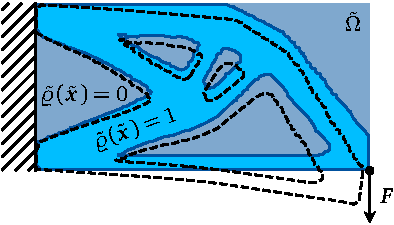
\includegraphics{topoOptExample_1}%
  \caption[%
    Example scenario for topology optimization%
  ]{%
    Example scenario for topology optimization.
    An object \emph{\textcolor{hellblau}{(light blue)}}
    is fixed on the left side
    of the object domain $\objdomain$
    \emph{\textcolor{mittelblau!50}{(darker blue)}}
    and deformed by a force $\force$, resulting in a displaced object
    \emph{(dashed).}
    The density function $\densglobal(\tilde{\*x})$ is one inside the object
    and zero outside.%
  }%
  \label{fig:topoOptExample}%
\end{SCfigure}



\subsection{Two-Scale Approach}
\label{sec:612twoScale}

\paragraph{Discretization and two-scale approach}

Of course, we cannot solve the problem \eqref{eq:topoOptProblemContinuous}
numerically,
as there are infinitely many density functions $\densglobal$.
For simplicity, we assume that $\objdomain$ is some hyper-rectangle
$\clint{\tilde{\*a}, \tilde{\*b}}
= \clint{\tilde{a}_1, \tilde{b}_1} \times \dotsb \times
\clint{\tilde{a}_{\dimobjdomain}, \tilde{b}_{\dimobjdomain}}$;
if it is not, we replace $\objdomain$ with its bounding box.
The object domain $\objdomain$ can then be split into
$M_1 \times \dotsb \times M_{\dimobjdomain}$
equally-sized and axis-aligned sub-hyper-rectangles,
which we call \term{macro-cells}
(where $M_1, \dotsc, M_{\dimobjdomain} \in \nat$).

In the \term{two-scale approach,}
we assume the material of the macro-cells to be
repetitions of infinitesimally small periodic structures
(i.e., identical for each macro-cell),
called \term{micro-cells.}
These micro-cells have a specific shape, which is parameterized by
$d$ \term{micro-cell parameters} $x_1, \dotsc, x_d$,
normalized to values in the unit interval $\clint{0, 1}$.
For instance, in two dimensions,
this shape may be an axis-aligned cross
with thicknesses $x_1$ and $x_2$, as shown in \cref{fig:twoScale}.
The choice of a suitable \term{micro-cell model}
(parametrization of the micro-cells)
depends on the optimization scenario and has to be done a priori.

\begin{figure}
  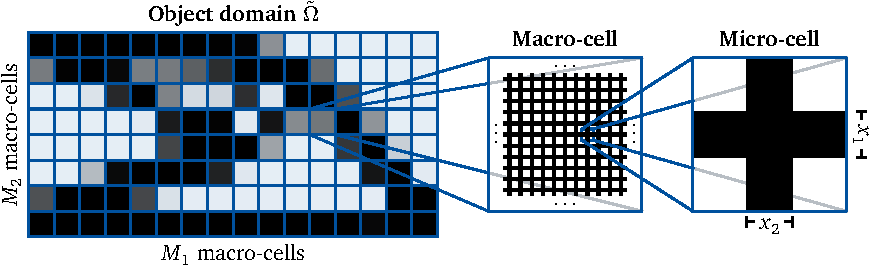
\includegraphics{twoScale_1}%
  \caption[%
    Two-scale approach for topology optimization%
  ]{%
    Two-scale approach to discretize the homogenized topology
    optimization problem in two dimensions ($\dimobjdomain = 2$).
    \emph{Left:} The object domain $\objdomain$ is
    subdivided into $M_1 \times M_2$ macro-cells,
    each with its own density \emph{(gray squares).}
    \emph{Center:} Every macro-cell is the repetition of infinitesimally small
    periodic micro-cells.
    \emph{Right:} The shape of the structure in every micro-cell is
    described by a micro-cell model with $d$ parameters $x_1, \dotsc, x_d$.
    Here, the micro-cell model is a cross with two parameters
    that represent the thickness of each crossbar.%
  }%
  \label{fig:twoScale}%
\end{figure}

\paragraph{Elasticity tensors}

Note that while the shape of all micro-cells in one macro-cell is identical,
the micro-cell parameters corresponding to different macro-cells differ
in general.
This enables varying densities in different regions of $\objdomain$.
We denote the micro-cell parameters corresponding to the $q$-th macro-cell
with $\mcp{q} = (\mcpentry{1}{q}, \dotsc, \mcpentry{d}{q}) \in
\clint{\*0, \*1} = \clint{0, 1}^d$,
where $q = 1, \dotsc, M$ and
$M \ceq M_1 \dotsm M_{\dimobjdomain}$ is the number of macro-cells.
With linear elasticity,
one can compute so-called \term{elasticity tensors} $\etensor^{(q)}$,
which encode information about the material properties
of the different macro-cells.
The elasticity tensors can be written as symmetric matrices
in $\real^{3 \times 3}$ (for $\dimobjdomain = 2$) or
in $\real^{6 \times 6}$ (for $\dimobjdomain = 3$).%
\footnote{%
  In general, the elasticity tensor is a fourth-order tensor in
  $\real^{\dimobjdomain \times \dimobjdomain \times \dimobjdomain \times \dimobjdomain}$.
  One can reduce the size of the tensor by exploiting various symmetries
  \cite{Huebner14Mehrdimensionale}
  to obtain $6$ or $21$ stiffness coefficients
  in two or three dimensions, respectively.
  These coefficients can then be expressed as a symmetric matrix.%
}
To simplify the following considerations,
we assume that $\dimobjdomain = 3$, i.e.,
$\etensor^{(q)} \in \real^{6 \times 6}$.
The elasticity tensors are usually computed as the solution of a \fem problem
\term{(micro-problem).}
Once all $\etensor^{(q)}$ are known,
we can compute the compliance value
by solving another \fem problem \term{(macro-problem),}
see \cite{Allaire04Topology} and \cite{Huebner14Mehrdimensionale}.

\vspace{-0.5em}

\paragraph{Discretized optimization problem}

The new optimization problem emerging from the
two-scale discretization process has the form
\begin{subequations}
  \label{eq:topoOptProblemDiscrete}
  \setlength{\belowdisplayskip}{5pt}%
  \begin{gather}
    \min J(\mcp{1}, \dotsc, \mcp{M}),\quad
    \mcp{1}, \dotsc, \mcp{M} \in \clint{\*0, \*1}
    \quad\text{s.t.}\quad
    \densmean(\mcp{1}, \dotsc, \mcp{M}) \le \densub,\\
    \densmean(\mcp{1}, \dotsc, \mcp{M})
    \ceq \frac{1}{M} \sum_{q=1}^M \denscell^{(q)}(\mcp{q}).
  \end{gather}
\end{subequations}
Here, $\denscell^{(q)}(\mcp{q}) \in \clint{0, 1}$ is the
density of the $q$-th macro-cell with micro-cell parameter $\mcp{q}$
(i.e., the fraction of material volume of one micro-cell
with respect to its total volume)
and $\densmean(\mcp{1}, \dotsc, \mcp{M}) \in \clint{0, 1}$
is the resulting total mean density.
This discretized optimization problem can now be implemented and
solved numerically.

\section{Approximating Elasticity Tensors}
\label{sec:62tensors}

\paragraph{Optimization process}

\minitoc{75mm}{7}

During the process of solving \cref{eq:topoOptProblemDiscrete},
optimization algorithms typically
evaluate the objective function $\compliance(\mcp{1}, \dotsc, \mcp{M})$
iteratively at different \term{micro-cell parameter combinations}
$(\mcp{1}, \dotsc, \mcp{M}) \in (\real^d)^M$.
Every evaluation of $\compliance$ corresponds to one solution of a
macro-problem.
However, to solve the macro-problem,
the elasticity tensors $\etensor^{(q)}$ of all $M$ macro-cells
need to be known.
Hence, in every optimization iteration, it is necessary to solve
one macro-problem and $M$ micro-cell problems,
all with the \fem.
This naive approach has two major drawbacks, which we explain in
the following.



\subsection{Drawbacks of the Naive Approach}
\label{sec:621drawbacks}

\paragraph{Drawback 1: Computation time}

First, this approach is computationally infeasible
even for simple micro-cell models and optimization scenarios.
The computation of a single elasticity tensor usually takes seconds to
minutes.
All $M$ micro-cell problems per optimization iteration
can be solved in parallel without any communication.
However, $M$ is typically in the range of thousands and
there are thousands or tens of thousands optimization iterations
(the optimization problem is $(d \cdot M)$-dimensional!).
This implies that the overall computation may still take
several days or even weeks to complete.

\paragraph{Drawback 2: Approximation of gradients}

Second, most optimization algorithms require gradients of the
objective function and of the constraints, i.e.,%
\begin{equation}
  \partialderiv{\partialdiff{} x_t}{\etensor^{(q)}}(\mcp{q}),\quad
  \partialderiv{\partialdiff{} x_t}{\denscell^{(q)}}(\mcp{q}),\qquad
  q = 1, \dotsc, M,\quad
  t = 1, \dotsc, d.
\end{equation}
However, in general, both gradients are unavailable and
have to be approximated by finite differences.
This introduces new error sources and
increases the number of elasticity tensors to be evaluated,
further slowing down the solution process.
Additionally, the number of optimization iterations necessary to
achieve convergence might increase
if there are discontinuities in the objective function
or its gradient.
Such discontinuities can already be caused by the inexact solution of the \fem.
If we need Hessians or other higher-order derivatives,
then the issues even worsen.



\subsection{B-Splines on Sparse Grids for Topology Optimization}
\label{sec:622BSplines}

\paragraph{Elasticity tensor function}

As a remedy, we replace the costly elasticity tensors with cheap surrogates.
If we assume that all macro-cells use the same micro-cell model,
the elasticity tensor $\etensor^{(q)}$ of the $q$-th macro-cell
with the parameter $\mcp{q} \in \clint{\*0, \*1}$
can be written as the value $\etensor(\mcp{q})$ of some function
$\etensor\colon \clint{\*0, \*1} \to \real^{6 \times 6}$
(assuming that $\dimobjdomain = 3$) at the point $\mcp{q}$.
In the following,
$\etensor\colon \clint{\*0, \*1} \to \real^m$
gives $m \in \nat$ values from which the symmetric elasticity tensor
can be uniquely reconstructed,
i.e., $m = 6$ for $\dimobjdomain = 2$ and $m = 21$ for $\dimobjdomain = 3$.
The vector-valued/matrix-valued versions of $\etensor$
will be used interchangeably.

\paragraph{Elasticity tensor surrogate}

The idea is to use B-splines on sparse grids to approximate
the elasticity tensor function $\etensor$.
In contrast to the theoretical framework that we established in
\cref{chap:20sparseGrids,chap:30BSplines,chap:40algorithms},
the function to be interpolated is not scalar-valued, but vector-valued.
This means that we have to construct $m$ sparse grid interpolants
$\etensorentryintp{j}$
for the $m$ components $\etensorentry{j}$ of $\etensor$ ($j = 1, \dotsc, m$).
Note that one could generate different spatially adaptive sparse grids for the
different components $\etensorentryintp{j}$.
However, it is not possible to evaluate only specific entries of $\etensor$
without also evaluating all other entries,
which means that we would waste computational resources by selecting only
a subset of the calculated entries.
Therefore, we use the same grid for all components.

Additionally, we approximate the density $\denscell^{(q)}$
of the $q$-th macro-cell with a surrogate $\denscellintp$ using
B-splines on the same sparse grid as for $\etensorentryintp{j}$
for reasons of implementation,
resulting in $m + 1$ sparse grid interpolants in total.
From a theoretical perspective, this is not necessary,
since the density can be explicitly calculated with simple formulas
for most micro-cell models, independently of evaluations of the
elasticity tensor.

\paragraph{Advantages}

Our approach has multiple obvious advantages:
\begin{itemize}
  \item
  The sparse grid interpolant $\etensorintp$ has to be generated only
  once in an \term{offline step} before the optimization algorithm starts.
  During the optimization \term{(online phase),}
  only inexpensive evaluations of $\etensorintp$ are performed,
  saving much computation time.
  
  \item
  Sparse grids ease the curse of dimensionality, which prohibits
  conventional full grid interpolation methods if $d > 4$.
  
  \item
  With spatially adaptive sparse grids and a suitable refinement criterion,
  we can spend more grid points in regions of interest of $\etensor$,
  e.g., regions with large oscillations.
  
  \item
  By using B-splines as basis functions,
  the interpolant $\etensorintp$ will be more accurate
  than with piecewise linear basis functions.
  In addition, we can calculate its derivatives
  $\tpartialderiv{\partialdiff{} x_t}{\etensorintp}(\mcp{q})$
  fast and explicitly,
  accelerating the speed of convergence of the optimizer.
\end{itemize}



\breakpagebeforenextheadingtrue
\subsection{Cholesky Factor Interpolation}
\label{sec:623cholesky}

\paragraph{Positive definiteness of elasticity tensors}

Unfortunately, just replacing elasticity tensors with
B-spline surrogates often does not lead to correct results in practice.
Experiments show that for only for some sparse grids,
the optimization algorithm converges to an optimal point
\cite{Valentin16Hierarchical}.
The optimization algorithm crashes for most spatially adaptive grids,
not being able to find any meaningful optimum.
%
The root of the problem proves to be that
the interpolated elasticity tensors $\etensorintp(\*x)$ are not
positive definite for specific
micro-cell parameters $\*x \in \clint{\*0, \*1}$.
However, indefinite or even negative definite tensors $\etensorintp$
would mimic unphysical behavior.%
\footnote{%
  In the scalar case, this is analogous to Hooke's law for linear springs,
  where the force $F = kx$ needed to displace the end of a spring
  (fixed at the other end) by $x$ is proportional to $x$.
  The proportionality constant $k$ (which corresponds to the elasticity tensor)
  has to be positive.%
}
Hence, it is imperative for the optimization process that
the interpolated elasticity tensors are \spd.

\paragraph{Positive definiteness of sparse grid interpolants}

Interpolation on sparse grids per se does not preserve
positive definiteness.
A counterexample is shown in \cref{fig:cholesky1},
which displays the minimal eigenvalue of the elasticity tensor surrogate
resulting from interpolation on a regular sparse grid.
As the positivity of the diagonal is a necessary condition
for positive definiteness,
small oscillations of the interpolant of some entries
already make the whole elasticity tensor non-positive-definite.

\begin{figure}
  \subcaptionbox{%
    Minimal eigenvalue of $\etensorintp(\*x)$%
    \label{fig:cholesky1}%
  }[65mm]{%
    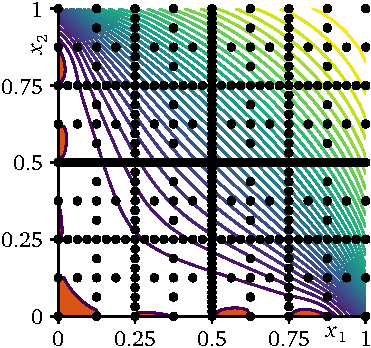
\includegraphics{cholesky_1}%
  }%
  \hfill%
  \subcaptionbox{%
    Minimal eigenvalue of $\etensorcholintp(\*x)$%
    \label{fig:cholesky2}%
  }[65mm]{%
    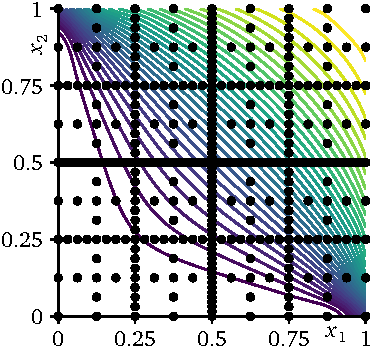
\includegraphics{cholesky_2}%
  }%
  \hfill\hfill%
  \raisebox{2.2mm}{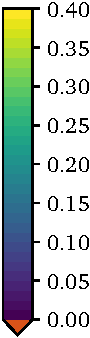
\includegraphics{cholesky_3}}%
  \caption[%
    Minimal eigenvalue of interpolated elasticity tensors%
  ]{%
    Minimal eigenvalue \emph{(colored contour lines)}
    of elasticity tensor surrogates
    for the 2D cross model ($\dimobjdomain = 2$, $d = 2$)
    \vspace{-0.3em}%
    and cubic hierarchical B-splines $\bspl{\*l,\*i}{p}$ ($p = 3$) on
    the regular sparse grid $\coarseregsgset{n}{d}{b}$ \emph{(dots)}
    with $n = 6$ and $b = 4$.
    \emph{Left:} The minimal eigenvalue of $\etensorintp(\*x)$
    becomes negative in some regions \emph{\textcolor{C1}{(red areas)}}
    of the domain $\clint{\*0, \*1}$,
    indicating that $\etensorintp(\*x)$ is not positive definite.
    \emph{Right:} The minimal eigenvalue of $\etensorcholintp(\*x)$
    is non-negative in the whole domain $\clint{\*0, \*1}$.%
  }%
  \label{fig:cholesky}%
\end{figure}

These oscillations are more likely to occur near the boundary of the domain
$\clint{\*0, \*1}$, such that there are larger regions
where the interpolated tensor is not positive definite anymore.
The reason is two-fold:
First, sparse grids without boundary points
are notoriously biased towards the center of the domain,
as they place only few points near the boundary \cite{Pflueger10Spatially}.
This leads to a loss of interpolation accuracy near the boundary
when compared to the center of $\clint{\*0, \*1}$.
Second, both the minimal eigenvalue of $\etensor(\*x)$ and the norm of its
gradient with respect to $\*x$ are small near $x_1 = 0$ or $x_2 = 0$.
Consequently, the ``surface'' of the minimal eigenvalue function
is rather flat in these regions and almost vanishes,
facilitating the existence of negative eigenvalues of
surrogate functions $\etensorintp(\*x)$.

Note that for most micro-cell models,
the optimization algorithm often evaluates the objective function
$\compliance(\mcp{1}, \dotsc, \mcp{M})$ at micro-cell parameter
combinations for which many of the points $\mcp{j}$ are near the boundary
of $\clint{\*0, \*1}$.
This is because many of the macro-cells will either be empty or
fully filled with material, which usually corresponds to micro-cell
parameters near zero or one, respectively.
Thus, $\etensorintp$ is frequently evaluated in the regions of
indefiniteness, which further worsens the issue.

\pagebreak

\paragraph{Positivity-preserving methods}

Even in one dimension, it cannot be guaranteed that the interpolant of
positive data remains positive,
which is a key problem in the estimation of probability densities
\multicite{Pflueger10Spatially,Griebel10Finite,Franzelin16From}.
Just clamping the interpolated values via $\max(\cdot, 0)$ does not help:
In our application, the tensor may still be indefinite;
additionally, the calculated gradients of the interpolants do not match
the actual gradients anymore.
In density estimation, clamping a density-like function changes its
integral, making it necessary to recalculate its normalization constant
\cite{Franzelin17Data}.

One possible workaround is to apply a continuous injective transformation
$T\colon \posreal \to \real$ on the positive values (e.g., $\ln$),
then interpolate the resulting values, and finally
apply the inverse transformation $T^{-1}\colon \real \to \posreal$
on the interpolated values (e.g., $\exp$).%
\footnote{%
  Formally, the inverse function $T^{-1}\colon T(\posreal) \to \posreal$
  is only defined on the image $T(\posreal)$ of $T$,
  which might not be the whole real line.
  However, we assume that $T^{-1}$ can be ``reasonably'' extended to $\real$
  (e.g., $T \ceq \sqrt{\cdot}$ and $T^{-1} = ({\cdot})^2$).%
}
For the piecewise linear hierarchical basis, another approach has been
developed recently \cite{Franzelin17Data},
maintaining the positivity by inserting additional sparse grid points.
In the context of spline approximation,
positivity-preserving approximation schemes based on so-called
quasi-interpolation are known \cite{Hoellig13Approximation}.
For our application, for which we need to preserve positive definiteness,
it is conceivable that one could apply these positivity-preserving
methods in the eigenspace,
interpolating the positive eigenvalues.

\paragraph{Interpolation of Cholesky factors}

Instead, we pursue a different, more canonical
approach based on Cholesky factorization:

\begin{proposition}[Cholesky factorization]
  For every \spd matrix $\etensor \in \real^{6 \times 6}$,
  there is a unique upper triangular matrix
  $\cholfactor \in \real^{6 \times 6}$
  with positive diagonal entries such that
  \begin{equation}
    \etensor
    = \tr{\cholfactor} \cholfactor.
  \end{equation}
\end{proposition}

\begin{proof}
  See \cite{Benoit24Note} or \cite{Freund07Stoer}.
\end{proof}

In one dimension, the Cholesky factorization is equivalent
to the application of a transformation $T$ as above by choosing
$T \ceq \sqrt{\cdot}$ and $T^{-1} = (\cdot)^2$.
Our approach is as follows:
\begin{enumerate}
  \item
  Define $\cholfactor\colon \clint{\*0, \*1} \to \real^{6 \times 6}$
  as the Cholesky factor of
  $\etensor\colon \clint{\*0, \*1} \to \real^{6 \times 6}$, i.e.,
  $\etensor(\*x) = \tr{\cholfactor(\*x)} \cholfactor(\*x)$
  for all $\*x \in \clint{\*0, \*1}$.
  
  \item
  During the grid generation (offline phase),
  evaluate $\etensor(\gp{\*l,\*i})$ at the grid points $\gp{\*l,\*i}$,
  compute the Cholesky factors $\cholfactor(\gp{\*l,\*i})$ of
  $\etensor(\gp{\*l,\*i})$,
  and interpolate them instead of the elasticity tensors
  to obtain an interpolant
  $\cholfactorintp\colon \clint{\*0, \*1} \to \real^{6 \times 6}$.
  
  \item
  During the optimization (online phase),
  every time the value $\etensor(\*x)$ of an elasticity tensor is needed,
  the interpolant $\cholfactorintp(\*x)$ is evaluated and we return
  \begin{equation}
    \etensorcholintp(\*x)
    \ceq \tr{\cholfactorintp(\*x)} \cholfactorintp(\*x).
  \end{equation}
\end{enumerate}

\paragraph{Advantages of Cholesky factor interpolation}

As shown in \cref{fig:cholesky2},
the resulting elasticity tensor surrogate $\etensorcholintp$
is positive semidefinite on the whole domain and
positive definite almost everywhere:
The surrogate $\etensorcholintp(\*x)$ is singular if and only if
$\cholfactorintp(\*x)$ is singular, which is in general
only the case on a negligible null set in $\clint{\*0, \*1}$.

Another advantage of this approach is that not only the
positive definiteness, but also the explicit differentiability
of the surrogate $\etensorcholintp$ is preserved.
The gradient can be computed easily and fast with the product rule:
\begin{equation}
  \label{eq:choleskyFactorDerivative}
  \partialderiv{\partialdiff{} x_t}{\etensorcholintp}(\*x)
  = \tr{\cholfactorintp(\*x)} \cdot
  \partialderiv{\partialdiff{} x_t}{\cholfactorintp}(\*x) +
  \tr{\partialderiv{\partialdiff{} x_t}{\cholfactorintp}(\*x)} \cdot
  \cholfactorintp(\*x),\quad
  t = 1, \dotsc, d,
\end{equation}
where both the sparse grid interpolant $\cholfactorintp(\*x)$ and
its derivative $\partialderiv{\partialdiff{} x_t}{\cholfactorintp}(\*x)$
are known.
As discussed above,
this is key to the applicability of gradient-based optimization.

\section{Micro-Cell Models and Optimization Scenarios}
\label{sec:63models}

\minitoc{62mm}{3}

\noindent
In the following, we present the different micro-cell models
and optimization scenarios for which we perform numerical
experiments in the next section.



\subsection{Micro-Cell Models}
\label{sec:631models}

We use the various micro-cell models that are depicted in \cref{fig:microCell}.
The models differ in the spatial dimensionality $\dimobjdomain$
and the number $d$ of micro-cell parameters
$\*x \in \clint{\*0, \*1} = \clint{0, 1}^d$.
Note that the presented models are only some examples.
One can easily design complicated micro-cell models
with larger numbers of parameters.

\begin{figure}
  \subcaptionbox{%
    \lefthphantom{2D cross}{(2D-C, $d = 2$)}\\(2D-C, $d = 2$)%
    \label{fig:microCell_1}%
  }[31mm]{%
    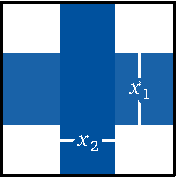
\includegraphics{microCell_1}%
  }%
  \hfill%
  \subcaptionbox{%
    2D framed cross\\(2D-FC, $d = 4$)%
    \label{fig:microCell_2}%
  }[31mm]{%
    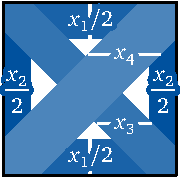
\includegraphics{microCell_3}%
  }%
  \hfill%
  \subcaptionbox{%
    2D sheared cross\\\rlap{\hspace*{11mm}{(2D-SC, $d = 3$)}}%
    \label{fig:microCell_3}%
  }[41mm]{%
    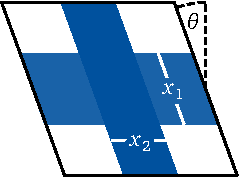
\includegraphics{microCell_2}%
  }%
  \hfill%
  \subcaptionbox{%
    2D sheared framed cross (2D-SFC, $d = 5$)%
    \label{fig:microCell_4}%
  }[37.5mm]{%
    \hspace*{-45mm}%
    \rlap{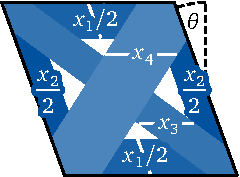
\includegraphics{microCell_4}}%
  }\\[2mm]%
  \subcaptionbox{%
    3D cross (3D-C, $d = 3$)%
    \label{fig:microCell_5}%
  }[44mm]{%
    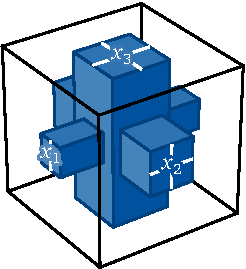
\includegraphics{microCell_5}%
  }%
  \quad%
  \subcaptionbox{%
    3D sheared cross (3D-SC, $d = 5$)%
    \label{fig:microCell_6}%
  }[56mm]{%
    \hspace*{5mm}%
    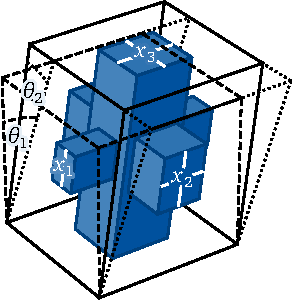
\includegraphics{microCell_6}%
  }%
  \caption[Types of micro-cell models]{%
    Types of micro-cell models in two dimensions \emph{(top row)}
    and three dimensions \emph{(bottom row)}.%
  }%
  \label{fig:microCell}%
\end{figure}

\paragraph{Orthogonal (non-sheared) models in two dimensions}

The basic component of the four two-dimensional models
is a square with a cross (\cref{fig:microCell_1})
of two axis-aligned orthogonal bars,
whose widths are determined by two micro-cell parameters $x_1$ and $x_2$.
The micro-cell parameters are ratios of the bar widths
to the edge lengths of the micro-cell
(although the actual micro-cells are infinitesimally small).
This results in the \emph{cross model.}
For the \term{framed cross model} (\cref{fig:microCell_2}),
we add a diagonal cross with orthogonal bars
of widths $x_3$ and $x_4$ (horizontally measured).
To simplify the boundary treatment,
we shift the contents of the framed cross micro-cell by
\SI{50}{\percent} of the micro-cell's edge lengths in both directions,
such that previous corners of the micro-cell correspond to the new center.

\paragraph{Sheared models in two dimensions}

Both of these models can be extended by shearing.
The idea is to increase the stability of the resulting macro-structure
with respect to forces that act at angles other than
\ang{0} and \ang{90} (cross model) or
\ang{0}, \ang{90}, and \ang{45} (framed cross model).
If we just rotated the crosses in the micro-cells,
then the micro-structure would not be periodic.
Instead, we shear the whole micro-cell in the horizontal direction,
where the shearing angle $\theta$ is an additional micro-cell parameter,
which gives us another degree of freedom.%
\footnote{%
  To be more precise, the angle $\theta$ corresponds to an
  additional micro-cell parameter $x_3$ (sheared cross) or
  $x_5$ (sheared framed cross) that is determined by normalization
  from $\clint{-0.35\pi, 0.35\pi}$, i.e., $\theta/(0.7\pi) + 1/2$.%
}
This results in the \term{sheared cross model} (\cref{fig:microCell_3})
and \term{sheared framed cross model} (\cref{fig:microCell_4})
with three and five micro-parameters each.

\paragraph{Models in three dimensions}

The two-dimensional cross model can be transferred to three
spatial dimensions by just adding another bar in the new dimension.
Each of the three bars has square cross-section with given edge lengths
$x_1$, $x_2$, or $x_3$, respectively,
resulting in the \term{3D cross model} with three micro-cell parameters
(\cref{fig:microCell_5}).
By shearing in the two horizontal directions,
we obtain two new degrees of freedom $\theta_1$ and $\theta_2$
(shearing angles).
The emerging \term{3D sheared cross model} has five micro-cell parameters
(\cref{fig:microCell_6}).



\subsection{Test Scenarios}
\label{sec:632scenarios}

To benchmark the performance of the new method,
we take a subset of the scenarios given in \cite{Valdez17Topology},
which reviews more than 100 papers on topology optimization
to determine the most common test scenarios in the field.
The geometry and the boundary conditions of the
four scenarios (two for each 2D and 3D)
are given in \cref{fig:topoOptScenario} (dimensions in meters).
In contrast to \cite{Valdez17Topology},
we only use single-point loads
(i.e., not loads applied to line segments, areas, or volumes)
for implementational reasons.
The upper bound on the density (see \cref{sec:611homogenization})
is $\densub = \SI{50}{\percent}$ for the 2D scenarios and
$\densub = \SI{10}{\percent}$ for the 3D scenarios.
As in \cite{Sigmund01Line} and for reasons of simplicity,
we apply a force $\force$ with unit value
(i.e., $\norm[2]{\force} = \SI{1}{\newton}$),
and we use a hypothetical material with
a Young's modulus (stiffness) of \SI{1}{\pascal} and
a Poisson ratio (transversal expansion to axial compression) of $0.3$.

\begin{figure}
  \subcaptionbox{%
    2D cantilever%
    \label{fig:topoOptScenario_1}%
  }[72mm]{%
    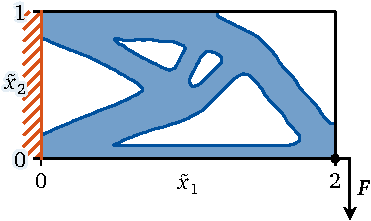
\includegraphics{topoOptScenario2D_1}%
  }%
  \hfill%
  \smash{\raisebox{-22mm}{\subcaptionbox{%
    2D L-shape%
    \label{fig:topoOptScenario_2}%
  }[72mm]{%
    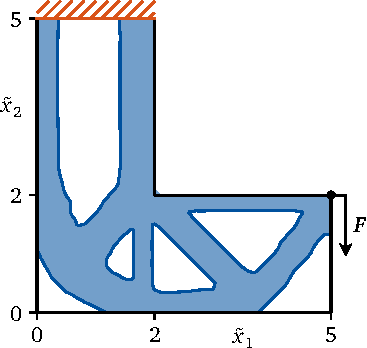
\includegraphics{topoOptScenario2D_2}%
  }}}%
  \\[7mm]%
  \subcaptionbox{%
    3D cantilever%
    \label{fig:topoOptScenario_3}%
  }[72mm]{%
    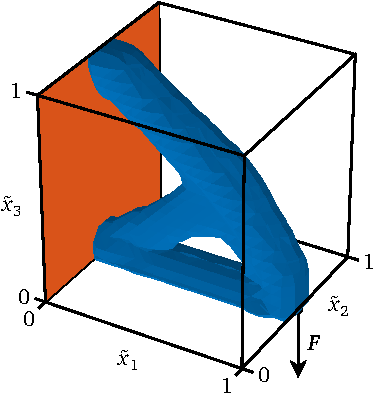
\includegraphics{topoOptScenario3D_1}%
  }%
  \hfill%
  \subcaptionbox{%
    3D center-load%
    \label{fig:topoOptScenario_4}%
  }[72mm]{%
    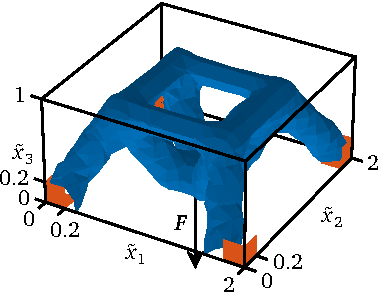
\includegraphics{topoOptScenario3D_2}%
  }%
  \caption[Test scenarios in topology optimization]{%
    Test scenarios in topology optimization in
    two and three spatial dimensions.
    Shown are
    the domains $\objdomain$,
    load points,
    locations of homogeneous Dirichlet boundary conditions
    \emph{\textcolor{C1}{(red)},} and
    exemplary optimal structures \emph{\textcolor{C0}{(blue)}.}%
  }%
  \label{fig:topoOptScenario}%
\end{figure}

\section{Implementation and Numerical Results}
\label{sec:64results}

\minitoc[-3mm]{73mm}{5}

\noindent
In this final section of the chapter,
we study optimal results of the test scenarios and
analyze interpolation errors and optimization results
for topology optimization with B-spline surrogates on sparse grids.



\subsection{Implementation}
\label{sec:641implementation}

In the following, for simplicity,
we combine the two functions to be interpolated,
i.e., the Cholesky factor
$\cholfactor\colon \clint{\*0, \*1} \to \real^{6 \times 6}$ and
the micro-cell density $\denscell\colon \clint{\*0, \*1} \to \real$,
to one single objective function
$\*\objfun\colon \clint{\*0, \*1} \to \real^{m+1}$,
from which both functions can be recovered.

\paragraph{Overview of offline and online phase}

Our method is divided into an offline phase and an online phase,
both of which are sketched in \cref{fig:topoOptPhases}.
The offline phase consists of
generating the spatially adaptive sparse grid
$\sgset = \{\gp{\*l_k,\*i_k} \mid k = 1, \dotsc, \ngp\}$,
solving the corresponding micro-problems,
computing the Cholesky factors, and
hierarchizing the Cholesky factor entries and micro-cell densities
to obtain the sparse grid interpolant $\vsgintp$.
Each optimization iteration of the online phase consists of
evaluating the interpolant $\vsgintp$
for each micro-cell parameter $\mcp{j}$ ($j = 1, \dotsc, M$),
reconstructing the elasticity tensor $\etensorcholintp$ from
the Cholesky factors $\cholfactorintp$,%
\footnote{%
  In addition, the partial derivatives
  $\partialdiff{} \etensorcholintp/\partialdiff{} x_t$
  ($t = 1, \dotsc, d$)
  are evaluated using \cref{eq:choleskyFactorDerivative}.
  This is necessary to employ gradient-based optimization.%
}
and solving the macro-problem to retrieve the approximated compliance value
$\complianceintp(\mcp{1}, \dotsc, \mcp{M})$.
The superscript in $\complianceintp$ indicates that
we do not use the exact elasticity tensors $\etensor$
to compute the compliance value,
but rather the reconstructed and interpolated tensors
$\etensorcholintp$.

\begin{figure}
  \tikzset{
    myCircle/.style={
      circle,
      fill=mittelblau!30,
      draw=mittelblau,
      inner sep=0.5mm,
    }
  }%
  \subcaptionbox{%
    Offline phase (without the actual grid generation).%
  }[149mm]{%
    \begin{tikzpicture}
      \node[myCircle] (points) at (0mm,0mm) {%
        $
          \begin{matrix}
            \gp{\*l_1,\*i_1},\\
            \dots,\\
            \gp{\*l_{\ngp},\*i_{\ngp}}
          \end{matrix}
        $%
      };
      \node[myCircle] (elasticityTensors) at (43mm,0mm) {%
        $
          \begin{matrix}
            \etensor(\gp{\*l_1,\*i_1}),\\
            \dots,\\
            \etensor(\gp{\*l_{\ngp},\*i_{\ngp}})
          \end{matrix}
        $%
      };
      \node[myCircle] (choleskyFactors) at (80mm,0mm) {%
        $
          \begin{matrix}
            \cholfactor(\gp{\*l_1,\*i_1}),\\
            \dots,\\
            \cholfactor(\gp{\*l_{\ngp},\*i_{\ngp}})
          \end{matrix}
        $%
      };
      \node[myCircle] (choleskyInterpolant) at (118mm,0mm) {%
        $
          \begin{matrix}
            \cholfactorintp\colon \clint{\*0, \*1}\\
            {} \to \real^{6 \times 6}
          \end{matrix}
        $%
      };
      \draw[->,draw=C0] (points) -- node[above] {%
        \footnotesize{}micro-problem%
      } (elasticityTensors);
      \draw[->,draw=C0] (elasticityTensors) -- node[above] {%
        \footnotesize{}%
        $
          \tr{\cholfactor} \cholfactor = \etensor
        $\vphantom{p}%
      } (choleskyFactors);
      \draw[->,draw=C0] (choleskyFactors) -- node[above] {%
        \footnotesize{}interpolate%
      } (choleskyInterpolant);
    \end{tikzpicture}%
  }%
  \\[2mm]%
  \subcaptionbox{%
    Online phase (one iteration of the optimizer).%
  }[149mm]{%
    \begin{tikzpicture}
      \node[myCircle] (points) at (0mm,0mm) {%
        $
          \begin{matrix}
            \mcp{1},\\
            \dots,\\
            \mcp{M}
          \end{matrix}
        $%
      };
      \node[myCircle] (choleskyFactors) at (34mm,0mm) {%
        $
          \begin{matrix}
            \cholfactorintp(\mcp{1}),\\
            \dots,\\
            \cholfactorintp(\mcp{M})
          \end{matrix}
        $%
      };
      \node[myCircle] (elasticityTensors) at (83mm,0mm) {%
        $
          \begin{matrix}
            \etensorcholintp(\mcp{1}),\\
            \dots,\\
            \etensorcholintp(\mcp{M})
          \end{matrix}
        $%
      };
      \node[myCircle] (complianceValue) at (129.5mm,0mm) {%
        $
          \begin{matrix}
            \complianceintp(\mcp{1},\\
            \dotsc,\\
            \mcp{M})
          \end{matrix}
        $%
      };
      \draw[->,draw=C0] (points) -- node[above] {%
        \footnotesize{}evaluate\vphantom{p}%
      } (choleskyFactors);
      \draw[->,draw=C0] (choleskyFactors) -- node[above] {%
        \footnotesize{}%
        $
          \etensorcholintp
          = \tr{(\cholfactorintp)} \cholfactorintp
        $\vphantom{p}%
      } (elasticityTensors);
      \draw[->,draw=C0] (elasticityTensors) -- node[above] {%
        \footnotesize{}macro-problem%
      } (complianceValue);
    \end{tikzpicture}%
  }%
  \caption[Offline and online phase for topology optimization]{%
    Offline and online phase for topology optimization.
    The interpolation of the
    micro-cell density $\denscell$ with $\denscellintp$
    (see \cref{sec:622BSplines}) has been omitted for brevity.%
  }%
  \label{fig:topoOptPhases}%
\end{figure}

\paragraph{Generation of spatially adaptive sparse grids}

We use the classical surplus-based refinement criterion
(see, e.g., \cite{Pflueger10Spatially})
as shown in \cref{alg:topoOptGridGeneration}
to generate the spatially adaptive sparse grids.
The difference to common surrogate settings is that the objective function
$\*f\colon \clint{\*0, \*1} \to \real^{m+1}$ is vector-valued.
As the entries of $\cholfactor$ cannot be evaluated individually,
the adaptivity criterion has to consider all entries at once
to avoid performing unnecessary evaluations.
We use the surpluses in the piecewise linear hierarchical basis,
as their absolute values correlate with the second mixed derivative
of the objective function due to \cref{eq:surplusIntegral}.
The surpluses are combined using the formula
$\beta_k \ceq \tr{\*c} \vabs{\vsurplus_{\*l_k,\*i_k}}$
(with entry-wise absolute value) and the
points with largest $\beta_k$ are refined.

\begin{algorithm}
  \begin{algorithmic}[1]
    \Function{$\sgset = \texttt{offlinePhase}$}{%
      $\*\objfun$, $n$, $b$, $\*c$, $l_{\max}$, $\refinetol$,
      $\ngp_{\mathrm{refine}}$%
    }
      \State{$\sgset \gets \coarseregsgset{n}{d}{b}$}
      \Comment{initial regular sparse grid}%
      \While{\True}
        \State{$\ngp \gets \setsize{\sgset}$}
        \Comment{number of grid points}%
        \State{%
          Let $(\vsurplus_{\*l_{k'},\*i_{k'}})_{k' = 1, \dotsc, \ngp}$
          satisfy $
            \fa{k = 1, \dotsc, \ngp}{
              \sum_{k'=1}^{\ngp} \vsurplus_{\*l_{k'},\*i_{k'}}
              \bspl{\*l_{k'},\*i_{k'}}{1}(\gp{\*l_k,\*i_k})
              = \*\objfun(\gp{\*l_k,\*i_k})
            }
          $%
        }
        \ForOneLine{$k = 1, \dotsc, \ngp$}{%
          $\beta_k \gets \tr{\*c} \vabs{\vsurplus_{\*l_k,\*i_k}}$%
        }
        \Comment{combine surpluses to a scalar value}%
        \State{%
          $
            \liset^\ast \gets \{
              k = 1, \dotsc, \ngp \mid
              \ex{\gp{\*l,\*i} \notin \sgset}{
                \gp{\*l_k,\*i_k} \to \gp{\*l,\*i}
              },\,
              \norm[\infty]{\*l_k} < l_{\max},\,
              \abs{\beta_k} > \refinetol
            \}
          $%
        }
        \IfOneLine{$\liset^\ast = \emptyset$}{\Break{}}
        \Comment{stop when there are no refinable grid points left}%
        \State{%
          Refine $\le \ngp_{\mathrm{refine}}$ of the points
          $\{\gp{\*l_k,\*i_k} \in \sgset \mid k \in \liset^\ast\}$
          with largest $\beta_k$%
        }
      \EndWhile{}
    \EndFunction{}
  \end{algorithmic}
  \caption[%
    Generation of spatially adaptive sparse grids for topology optimization%
  ]{%
    Generation of spatially adaptive sparse grids for topology optimization.
    Inputs are
    the objective function $\*f\colon \clint{\*0, \*1} \to \real^{m+1}$
    (combination of the Cholesky factor of the elasticity tensor and
    the micro-cell density),
    the level $n \ge d$ and boundary parameter $b \in \nat$ of the
    initial regular sparse grid,
    the vector $\*c \in \real^{m+1}$ of coefficients with which the
    absolute values of the entries of the surpluses are combined,
    the maximal level $l_{\max} \in \nat$,
    the refinement threshold $\refinetol \in \posreal$, and
    the number $\ngp_{\mathrm{refine}} \in \nat$ of points to refine
    in each iteration.
    Output is the spatially adaptive sparse grid $\sgset$.%
  }%
  \label{alg:topoOptGridGeneration}%
\end{algorithm}

\paragraph{Parameter bounds}

In the micro-cell models presented in \cref{sec:631models},
extreme micro-cell parameters near zero or one may cause problems
with the resulting elasticity tensors.
For instance, many elasticity tensor entries corresponding to
the 2D cross model are discontinuous near the lines $x_1 = 1$ or $x_2 = 1$
\multicite{Huebner14Mehrdimensionale,Valentin14Hierarchische}.
This is due to the fact that the micro-cell is completely filled with material
on these lines,
independent of the other micro-cell parameter.
Similar issues occur for the other models and the shearing angles.
Hence, we have to restrict the range of the feasible micro-cell parameters,
i.e., the sparse grid points
$\*x = \gp{\*l_k,\*i_k}$ are still defined on the unit hyper-cube
$\clint{\*0, \*1}$,
but the actual micro-cell parameters $\xscaled$ are retrieved by an
affine transformation $\xscaled \ceq \*a + (\*b - \*a) \*x$.
For the models in \cref{sec:631models},
we restrict the bar widths to $\clint{0.01, 0.99}$ and
the shearing angles to $\clint{-0.35\pi, 0.35\pi}$.

\paragraph{Software, algorithms, and domain discretization}

The micro-problems and macro-problems were solved with the
\fem software package CFS++ \cite{Kaltenbacher10Advanced}.%
\footnote{%
  \url{http://www.lse.uni-erlangen.de/cfs/}%
}
The micro-prob\-lems were discretized by dividing the micro-cells into
$128 \times 128 = \num{16384}$ elements (models in two dimensions) or
$16 \times 16 \times 16 = \num{4096}$ elements (models in three dimensions).
The macro-domains $\objdomain$ were discretized using
32 macro-cells per meter in the 2D cantilever scenario
(i.e., $64 \times 32 = \num{2048}$ cells),
20 macro-cells per meter in the 3D cantilever scenario
(i.e., $20 \times 20 \times 20 = \num{8000}$ cells), and
10 macro-cells per meter in the other scenarios
(i.e.,
\num{1600} cells for the 2D L-shape and
\num{4000} cells for the 3D center-load).
The generation of the sparse grids (offline phase) was done via a MATLAB code,
while the evaluation of the interpolants (online phase) was performed
by the sparse grid toolbox \sgpp \cite{Pflueger10Spatially}.%
\footnote{%
  \url{http://sgpp.sparsegrids.org/}%
}
For the solution of the emerging optimization problems,
a sequential quadratic programming method was employed
(see \cref{sec:513gradientBasedConstrained}).



\subsection{Error Sources}
\label{sec:642errorSources}

There are multiple sources that contribute to the numerical error
of our method:

\begin{enumerate}[label=E\arabic*.,ref=E\arabic*,leftmargin=2.7em]
  \item
  \label{item:topoOptErrorMicro}
  Discretization of the micro-problem
  (i.e., the elasticity tensors $\etensor$ are inaccurate)
  
  \item
  \label{item:topoOptErrorInterpolation}
  Sparse grid interpolation
  (i.e., $\etensorintp \not= \etensor$)
  
  \item
  \label{item:topoOptErrorCholesky}
  Reconstruction of elasticity tensors with Cholesky factors
  (i.e., $\etensorcholintp \not= \etensorintp$)
  
  \item
  \label{item:topoOptErrorMacro}
  Discretization of the macro-problem
  (i.e., the compliance $\compliance$ is inaccurate)
  
  \item
  \label{item:topoOptErrorOptimization}
  Optimization
  (i.e., the minimum found by the optimizer is inaccurate or not global)
  
  \item
  \label{item:topoOptErrorRounding}
  Floating-point rounding errors
  (i.e., arithmetical operations are inaccurate)
\end{enumerate}

\noindent
\ref{item:topoOptErrorRounding}-type errors are always present and
will not be analyzed in this chapter.
Errors of type \ref{item:topoOptErrorMicro} and \ref{item:topoOptErrorMacro}
are intrinsic to the homogenization approach
and will not be discussed here either.
The optimization error \ref{item:topoOptErrorOptimization}
has already been discussed in \cref{sec:542optimization}
for explicit test functions.
Therefore, in the remainder of this chapter,
we will focus on the analysis of the errors of types
\ref{item:topoOptErrorInterpolation} and \ref{item:topoOptErrorCholesky},
since the interpolation of Cholesky factors is the
major new contribution to this application.



\subsection{Interpolation Error}
\label{sec:643interpolation}

\paragraph{Spectral interpolation error measure}

For the interpolation error \ref{item:topoOptErrorInterpolation} and
the Cholesky factorization error \ref{item:topoOptErrorCholesky},
we cannot simply take the absolute value of the difference
of the objective function $\*\objfun\colon \clint{\*0, \*1} \to \real^{m+1}$
and its surrogate $\vsgintp$, since both are vector-valued.
As the micro-cell density $\denscell$
is not affected by the Cholesky factorization,
we consider only the elasticity tensor
$\etensor\colon \clint{\*0, \*1} \to \real^{6 \times 6}$ and
its surrogate
$\etensorcholintp\colon \clint{\*0, \*1} \to \real^{6 \times 6}$
obtained by Cholesky factorization.
To retrieve a scalar error measure,
we use the spectral norm
\begin{equation}
  \norm[2]{\etensor(\*x) - \etensorcholintp(\*x)},\quad
  \*x \in \clint{\*0, \*1},
\end{equation}
i.e., the largest absolute eigenvalue of
$\etensor(\*x) - \etensorcholintp(\*x)$.
However, the choice of the norm is arbitrary,
as all matrix norms on $\real^{6 \times 6}$ are equivalent to each other.

\paragraph{Pointwise spectral interpolation error}

\Cref{fig:topoOptInterpolationErrorPointwise}
shows the pointwise spectral interpolation error for the 2D cross model
and the corresponding spatially adaptive sparse grid
generated with the refinement algorithm as explained in
\cref{sec:641implementation}.
The above-mentioned discontinuity of elasticity tensor entries
near $x_1 = 1$ or $x_2 = 1$
is most severe near the corners $\*x \in \{(0, 1), (1, 0)\}$
(cf.\ \cref{fig:cholesky}),
as some entries vanish if one of the micro-cell bars has zero width.
Hence, most points are placed near these singularity corners.

\begin{figure}
  \subcaptionbox{%
    $\norm[2]{\etensor(\*x) - \etensorintp(\*x)}$%
    \label{fig:topoOptInterpolationErrorPointwise_1}%
  }[63mm]{%
    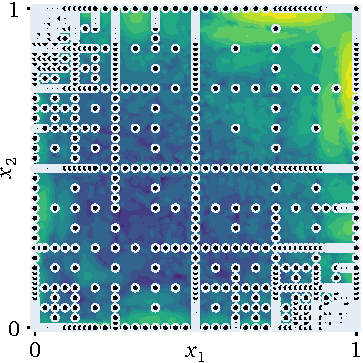
\includegraphics{topoOptInterpolationPointwise_1}%
  }%
  \hspace{3mm}%
  \subcaptionbox{%
    $\norm[2]{\etensor(\*x) - \etensorcholintp(\*x)}$%
    \label{fig:topoOptInterpolationErrorPointwise_2}%
  }[63mm]{%
    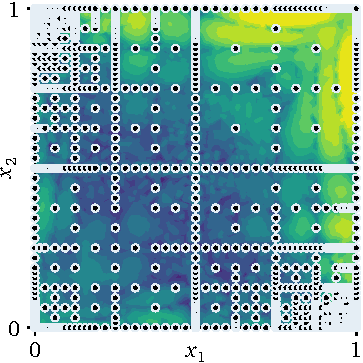
\includegraphics{topoOptInterpolationPointwise_2}%
  }%
  \hfill%
  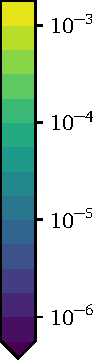
\includegraphics{topoOptInterpolationPointwise_3}%
  \caption[Pointwise spectral interpolation error for the 2D cross model]{%
    Pointwise spectral interpolation error for the 2D cross model and
    cubic B-splines on
    $\ngp = 1320$ spatially adaptive sparse grid points \emph{(dots)} for
    the direct elasticity tensor interpolation \emph{(left)} and
    the Cholesky factor interpolation \emph{(right).}%
  }%
  \label{fig:topoOptInterpolationErrorPointwise}%
\end{figure}

The left plot (\cref{fig:topoOptInterpolationErrorPointwise_1})
shows the spectral interpolation error
$\norm[2]{\etensor(\*x) - \etensorintp(\*x)}$
of the direct elasticity tensor interpolant without Cholesky factorization
(i.e., error \ref{item:topoOptErrorInterpolation}).
The maximum error is \num{1.2e-3},
which is attained near the critical lines $x_1 = 1$ or $x_2 = 1$.
Note that the mean error over the whole domain $\clint{\*0, \*1}$
is only \num{4.5e-5}.
In the right plot (\cref{fig:topoOptInterpolationErrorPointwise_2}),
the picture changes slightly when looking at the spectral interpolation error
$\norm[2]{\etensor(\*x) - \etensorcholintp(\*x)}$
of the elasticity tensor resulting from Cholesky factorization
(i.e., errors \ref{item:topoOptErrorInterpolation} and
\ref{item:topoOptErrorCholesky} combined).
The maximum error becomes \num{3.4e-3},
while the mean error increases to \num{1.1e-4}.
We conclude that the Cholesky factorization leads to an increase
of interpolation errors by only less than half an order of magnitude.

\paragraph{Convergence of spectral interpolation error}

\Cref{fig:topoOptInterpolationErrorBasisFunctions_1} shows
the convergence of the relative $\Ltwo$ spectral interpolation errors
\begin{equation}
  \error^{\sparse} \ceq
  \frac{
    \normLtwoscaled{
      \vphantom{\big(}
      \norm[2]{\etensor({\cdot}) - \etensorintp({\cdot})}
    }
  }{
    \normLtwoscaled{
      \vphantom{\big(}
      \norm[2]{\etensor({\cdot})}
    }
  }, \qquad
  \error^{\chol,\sparse} \ceq
  \frac{
    \normLtwoscaled{
      \vphantom{\big(}
      \norm[2]{\etensor({\cdot}) - \etensorcholintp({\cdot})}
    }
  }{
    \normLtwoscaled{
      \vphantom{\big(}
      \norm[2]{\etensor({\cdot})}
    }
  }
\end{equation}
for the 2D cross model, i.e.,
the relative $\Ltwo$ error of the functions depicted in
\cref{fig:topoOptInterpolationErrorPointwise}.
Relative errors of \SI{1}{\permille} are already obtained
for $\ngp = 200$ grid points.
Unfortunately, even for higher B-spline degrees $p > 1$,
the order of convergence is only quadratic
due to the singularities of the elasticity tensor.
This slow convergence does not improve for the other
micro-cell models as shown in
\Cref{fig:topoOptInterpolationErrorBasisFunctions_2}.
In fact, the convergence decelerates even more
as the number of micro-cell parameters increases.
For the 2D sheared cross and 3D cross models with three parameters,
the spatially adaptive sparse grid with $\ngp \approx \num{10000}$ grid points
is able to achieve a relative error of around \SI{3}{\permille}.
However, for the 2D sheared framed cross and 3D sheared cross models
with five parameters, only errors of about \SI{5}{\percent} are reached
for the same grid size.

\begin{figure}
  \hspace*{5mm}%
  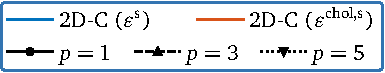
\includegraphics{topoOptInterpolation_3}%
  \hfill%
  \raisebox{0.5mm}{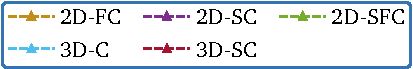
\includegraphics{topoOptInterpolation_4}}%
  \\[2mm]%
  \subcaptionbox{%
    $\error^{\sparse}$ \emph{\textcolor{C0}{(blue)}} and
    $\error^{\chol,\sparse}$ \emph{\textcolor{C1}{(red)}}
    for the 2D cross model and different degrees.%
    \label{fig:topoOptInterpolationErrorBasisFunctions_1}%
  }[72mm]{%
    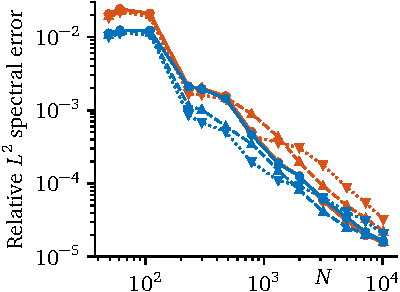
\includegraphics{topoOptInterpolation_1}%
  }%
  \hfill%
  \subcaptionbox{%
    $\error^{\chol,\sparse}$
    for the other models and $p = 3$.%
    \label{fig:topoOptInterpolationErrorBasisFunctions_2}%
  }[72mm]{%
    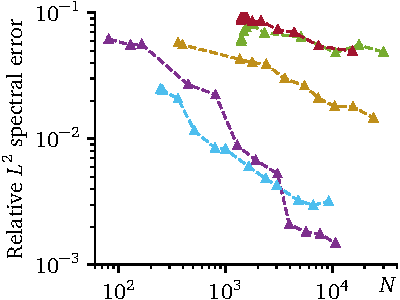
\includegraphics{topoOptInterpolation_2}%
  }%
  \caption[Convergence of relative $L^2$ spectral interpolation errors]{%
    Convergence of relative $\Ltwo$ spectral interpolation errors
    over the increasing number $\ngp$ of spatially adaptive grid points
    (i.e., decreasing threshold $\refinetol$)
    for the 2D cross model without or with Cholesky factor interpolation
    and different degrees $p$ \emph{(left)} and
    for the other models and cubic degree \emph{(right)}.%
  }%
  \label{fig:topoOptInterpolationErrorBasisFunctions}%
\end{figure}



\subsection{Optimal Compliance Values and Structures}
\label{sec:644optimization}

\paragraph{Optimal compliance values for different micro-cell models}

In the following, we use for each micro-cell model
a specific spatially adaptive sparse grid with around \num{10000} points.
The exact grid sizes and other details about the employed sparse grids
can be found in \cref{tbl:topoOptModels}
(located in \cref{chap:a30topoOptDetails}).
For hierarchical cubic B-splines ($p = 3$),
\cref{tbl:topoOptResultsModels} lists the
compliance values $\compliance(\mcpoptappr{1}, \dotsc, \mcpoptappr{M})$
for each of the four scenarios
and the corresponding possible micro-cell models,
where $(\mcpoptappr{1}, \dotsc, \mcpoptappr{M}) \in (\real^d)^M$
is the micro-cell parameter combination that is returned by the optimizer.%
\footnote{%
  Note that this true compliance value differs from the
  approximated value
  $\complianceintp(\mcpoptappr{1}, \dotsc, \mcpoptappr{M})$,
  which the optimizer reports as the optimal objective function value.%
}
It is obvious that more complicated micro-cell models
lead to lower (better) compliance values,
as they are a generalization of the simple models.
For instance, the 2D cross is a special case of
the 2D framed cross, the 2D sheared cross, and the 2D sheared framed cross.
By choosing the respectively best model for each scenario,
we are able to decrease the compliance value
(and, hence, increase the stability of the resulting structure)
by \SI{9.6}{\percent} in the 2D cantilever scenario,
by \SI{7.7}{\percent} in the 2D L-shape scenario,
by \SI{34}{\percent} in the 3D cantilever scenario, and
by \SI{73}{\percent} in the 3D center-load scenario.
In general, this motivates the usage of more complicated micro-cell models,
which cannot be computationally handled with
conventional full grid interpolation methods.
Consequently, sparse grids or similar methods have to be used.

\begin{table}
  \setnumberoftableheaderrows{1}%
  \begin{tabular}{%
    >{\kern\tabcolsep}=l<{\kern5mm}*{6}{+c}<{\kern\tabcolsep}%
  }
    \toprulec
    \headerrow
    Scenario&       2D-C&   2D-FC&  2D-SC&           2D-SFC& 3D-C&   3D-SC\\
    \midrulec
    2D cantilever&  74.974& 70.816& \textbf{67.809}& 68.602& ---&    ---\\
    2D L-shape&     183.68& 177.51& \textbf{169.60}& 174.55& ---&    ---\\
    \midrulec
    3D cantilever&  ---&    ---&    ---&             ---&    247.60& \textbf{162.59}\\
    3D center-load& ---&    ---&    ---&             ---&    169.27& \textbf{46.171}\\
    \bottomrulec
  \end{tabular}
  \caption[Optimal compliance values for different micro-cell models]{%
    Optimal compliance values for the different scenarios
    and micro-cell models using cubic B-splines
    (spatially adaptive grids with around \num{10000} points).
    The entries highlighted in \textbf{bold face} indicate the best choice
    of micro-cell models for a given scenario.
    More details can be found in \cref{tbl:topoOptResultsDetailed}.%
  }%
  \label{tbl:topoOptResultsModels}%
\end{table}

\paragraph{Corresponding optimal structures}

The corresponding optimal structures are shown in
\cref{fig:topoOptStructure2DCantilever} for the 2D cantilever scenario
and, for reasons of space, in \cref{chap:a30topoOptDetails} in
\cref{fig:topoOptStructure2DLShape,fig:topoOptStructure3D}
for the other three scenarios.
Of course, the periodic micro-cell structures cannot be plotted directly,
as the micro-cells are infinitesimally small.
Therefore, the figures show for each macro-cell only
one single large micro-cell.

\begin{figure}
  \subcaptionbox{%
    2D cross%
  }[72mm]{%
    
\includegraphics{topoOptStructure2D_1}%
  }%
  \hfill%
  \subcaptionbox{%
    2D framed cross%
  }[72mm]{%
    
\includegraphics{topoOptStructure2D_3}%
  }%
  \\[2mm]%
  \subcaptionbox{%
    2D sheared cross%
  }[72mm]{%
    
\includegraphics{topoOptStructure2D_5}%
  }%
  \hfill%
  \subcaptionbox{%
    2D sheared framed cross%
  }[72mm]{%
    
\includegraphics{topoOptStructure2D_7}%
  }%
  \caption[Optimal structures in the 2D cantilever scenario]{%
    Topologically optimal structures in the 2D cantilever scenario
    for different micro-cell models using cubic B-splines
    (spatially adaptive grids with around \num{10000} points).
    The colors indicate the length of the displacement,
    where dark regions correspond to weak displacements and
    bright regions to strong displacements.
    The color map is the same as in
    \cref{fig:topoOptStructure2DLShape}.
    Only bars with widths $\ge 0.1$ are shown.
    More details can be found in \cref{tbl:topoOptResultsDetailed}.%
  }%
  \label{fig:topoOptStructure2DCantilever}%
\end{figure}

Two effects can be seen in the plots of the optimal structures:
First, the simpler models are not able to direct the emerging forces at
arbitrary angles.
For example, the 2D framed cross model strongly prefers
angles of \ang{45}, which results in structures that are not as stable
as they could be.
The 2D sheared cross and 2D sheared framed cross models
are considerably more flexible, allowing
internal forces to act at almost arbitrary angles.
Second, the sheared micro-cell models use the available
material volume more efficiently than the cross model.
This is most striking in the 3D case (see \cref{fig:topoOptStructure3D}),
where it seems that the sheared cross structures
use more volume than the simple cross structures,
although the structures spend exactly the same amount of material volume.
The reason is that for the cross model, both bars
have to be used in order to connect the macro-cell to its neighbors.
For the sheared cross model, a shearing of the vertical bar suffices,
and we save volume by not using the horizontal bar.
Both of these effects explain the significantly lower compliance
values for the sheared micro-cell models.

\paragraph{Comparison to the direct solution}

B-splines on sparse grids lead to a drastic reduction in computation time.
Solving the 2D cantilever scenario with the best-placed sheared cross model
would take 453 days with
exact elasticity tensor evaluations (i.e., without surrogates),
assuming the same number of iterations as for the surrogate tensor case
and sequential computation of the elasticity tensors.
This estimate does not account for approximating the missing derivatives
of the elasticity tensor.
If we incorporate this and use 100 parallel processes,
we still need weeks for the solution.
In contrast, the computation time using our sparse grid surrogates
is a matter of minutes or hours at most,
resulting in speedups of around 200.
This is excluding the time for the offline phase,
which is in the range of hours, but which has to be spent only once,
as the resulting grid can be reused for different scenarios.

\vspace{2em}

\paragraph{Optimality-interpolation gaps}

\begin{figure}
  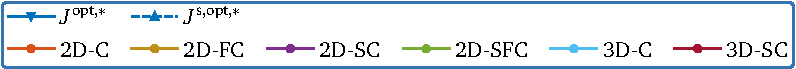
\includegraphics{topoOptOptimalityGap_3}%
  \\[2mm]%
  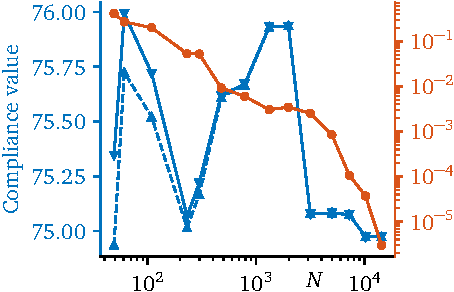
\includegraphics{topoOptOptimalityGap_1}%
  \hfill%
  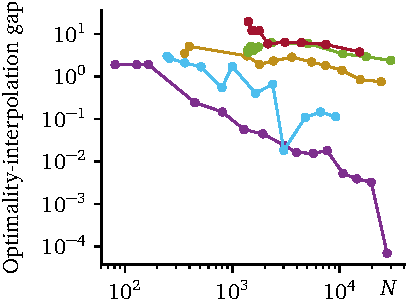
\includegraphics{topoOptOptimalityGap_2}%
  \caption[Convergence of the optimality-interpolation gap]{%
    Convergence of the optimality-interpolation gap
    $\abs{\compliance[\opt,\ast] - \complianceintp[\opt,\ast]}$
    for the 2D/3D cantilever scenario
    and different micro-cell models using cubic B-splines ($p = 3$).
    The left plot additionally shows
    $\compliance[\opt,\ast]
    \ceq \compliance(\mcpoptappr{1}, \dotsc, \mcpoptappr{M})$ and
    $\complianceintp[\opt,\ast]
    \ceq \complianceintp(\mcpoptappr{1}, \dotsc, \mcpoptappr{M})$
    for the 2D cross model.%
  }%
  \label{fig:topoOptOptimalityGap}%
\end{figure}

Ideally, we would measure the true optimality gap
\begin{equation}
  \label{eq:topoOptOptimalityGapTrue}
  \compliance(\mcpoptappr{1}, \dotsc, \mcpoptappr{M}) -
  \compliance(\mcpopt{1}, \dotsc, \mcpopt{M}),
\end{equation}
cf.\ error \ref{item:topoOptErrorOptimization}.
Unfortunately, the true optimum
$(\mcpopt{1}, \dotsc, \mcpopt{M})$ could not be computed:
Apart from the time issue mentioned above,
oscillations in the elasticity tensor evaluation and
errors stemming from types
\ref{item:topoOptErrorMicro} and \ref{item:topoOptErrorRounding}
reliably led to optimizer crashes as it ran into discontinuities,
which are smoothed out when using B-spline surrogates.
However, as in \cref{fig:topoOptOptimalityGap},
we can at least calculate the \term{optimality-interpolation gap}
\begin{equation}
  \label{eq:topoOptOptimalityGapPseudo}
  \abs{
    \compliance(\mcpoptappr{1}, \dotsc, \mcpoptappr{M}) -
    \complianceintp(\mcpoptappr{1}, \dotsc, \mcpoptappr{M})
  }
\end{equation}
between the actual compliance value
and the approximated, reported compliance value.
This gap does not constitute any kind of bound on the true optimality gap;
however, the idea is that
as the interpolation error converges to zero,
the optimality-interpolation gap should converge to zero, too.

\pagebreak

\Cref{fig:topoOptOptimalityGap} (left) shows that for the 2D cross model,
the optimizer reports compliance values that are smaller than in reality
($\complianceintp[\opt,\ast]$ vs. $\compliance[\opt,\ast]$).
However, the difference steadily converges to zero.
This is similar for the other micro-cell model as shown in the
right part of \cref{fig:topoOptOptimalityGap},
although the convergence is much slower due to the
higher number $d$ of micro-cell parameters.

\paragraph{Optimal compliance values for different B-spline degrees}

Finally, to study the effect of the B-spline degree on the
optimization performance,
\cref{tbl:topoOptResultsDegrees} lists the compliance values
for the degrees $p = 1, 3, 5$ and the 2D/3D cross and sheared cross
micro-cell models.
In the two-dimensional scenarios,
higher-order B-splines decrease the compliance value
by up to \SI{9}{\percent}.
In the three-dimensional scenarios,
higher-order B-splines may perform worse than the piecewise linear
functions ($p = 1$).
(However, as indicated in \cref{tbl:topoOptResultsDegrees},
all optimization runs with piecewise linear functions
terminated prematurely due to numerical difficulties with the
discontinuous derivatives.)
It may be suspected that if we used micro-cell models with
less prominent discontinuities (i.e., ``smoother'' elasticity tensors),
the advantage of higher-order B-splines would be more visible.
All in all, the application of topology optimization underlines
that good interpolation (and thus a good quality of the surrogate)
is key to good optimization results.

\begin{table}
  \setnumberoftableheaderrows{2}%
  \begin{tabular}{%
      >{\kern\tabcolsep}=l<{\kern5mm}*{3}{+c}%
      <{\kern5mm}*{3}{+c}<{\kern\tabcolsep}%
    }
    \toprulec
    \headerrow
    &
    \multicolumn{3}{c}{\hspace*{-12pt}2D/3D cross}&
    \multicolumn{3}{c}{\hspace*{-6pt}2D/3D sheared cross}\\
    \headerrow
    Scenario&       $p = 1$&         $p = 3$&         $p = 5$&          $p = 1$&                $p = 3$&         $p = 5$\\
    \midrulec
    2D cantilever&  \emph{82.365}&   \textbf{74.974}& 76.070&           \emph{68.889}&          \textbf{67.809}& 68.018\\
    2D L-shape&     \emph{193.83}&   \textbf{183.68}& 183.70&           \emph{169.85}&          169.60&          \textbf{169.60}\\
    \midrulec
    3D cantilever&  \emph{249.75}&   247.60&          \textbf{247.33}&  \emph{\textbf{148.72}}& 162.59&          152.34\\
    3D center-load& \textbf{162.68}& 169.27&          163.94&           \emph{\textbf{45.713}}& 46.171&          47.074\\
    \bottomrulec
  \end{tabular}
  \caption[Optimal compliance values for different B-spline degrees]{%
    Optimal compliance values for the different scenarios
    and B-spline degrees using the 2D/3D cross micro-cell model \emph{(left)}
    and the 2D/3D sheared cross micro-cell model \emph{(right).}
    The spatially adaptive sparse grids are the same as in
    \cref{tbl:topoOptResultsModels}.
    The entries highlighted in \textbf{bold face} indicate the best choice
    of B-spline degree for a given scenario and micro-cell model.
    Optimization runs of entries marked as \emph{italic}
    terminated prior to success due to numerical difficulties.%
  }%
  \label{tbl:topoOptResultsDegrees}%
\end{table}


\cleardoublepage
